\documentclass[12pt]{article}
\usepackage[margin=1cm]{geometry}
\usepackage{polski}
\usepackage[utf8]{inputenc}
\usepackage{siunitx}
\usepackage{amsmath}
\usepackage{graphicx}
\usepackage{multicol}
\usepackage{nopageno}
\usepackage{multirow}
\usepackage{csvsimple}

\renewcommand{\arraystretch}{1.3}

\newenvironment{Figure}
  {\par\medskip\noindent\minipage{\linewidth}}
  {\endminipage\par\medskip}

\title{\textbf{Współczynnik załamania światła - opracowanie danych}}
\author{}
\date{}

\begin{document}
\maketitle
\begin{multicols}{3}
\section{Szkło}
\csvreader[tabular=|c|c|c|c|,
    table head=\hline Nr & $h_g$ & $h_d$ & $\Delta_h$ \\\hline,
    late after line=\\\hline]%
{glass.csv}{hg=\hg,hd=\hd,dh=\dh}%
{\thecsvrow & \hg & \hd & \dh}
\\
\\
$\bar{\Delta_h} = \mathbf{2.514}$
\columnbreak

\section{Pleksiglas}
\csvreader[tabular=|c|c|c|c|,
    table head=\hline Nr & $h_g$ & $h_d$ & $\Delta_h$ \\\hline,
    late after line=\\\hline]%
{plexi.csv}{hg=\hg,hd=\hd,dh=\dh}%
{\thecsvrow & \hg & \hd & \dh}
\\
\\
$\bar{\Delta_h} = \mathbf{1.428}$
\columnbreak

\section{Filtry}
\begin{tabular}{|c|c|c|c|c|}
\hline
$\lambda$ & $h_g$ & $h_d$ & $\Delta_h$    & $\bar{\Delta_h}$   \\ \hline
\multirow{2}{*}{0.48} & 6.20 & 4.70 & 1.50 & \multirow{2}{*}{1.50} \\ \cline{2-4}
                      & 6.22 & 4.72 & 1.50 &                        \\ \hline
\multirow{2}{*}{0.63} & 6.21 & 4.72 & 1.49 & \multirow{2}{*}{1.53} \\ \cline{2-4}
                      & 6.27 & 4.70 & 1.57 &                        \\ \hline
\multirow{2}{*}{0.59} & 6.21 & 4.73 & 1.48 & \multirow{2}{*}{1.49}  \\ \cline{2-4}
                      & 6.19 & 4.69 & 1.50 &                        \\ \hline
\multirow{2}{*}{0.50} & 6.25 & 4.71 & 1.54 & \multirow{2}{*}{1.52}  \\ \cline{2-4}
                      & 6.20 & 4.70 & 1.50 &                        \\ \hline
\end{tabular}

\end{multicols}
\begin{Figure}
\centering
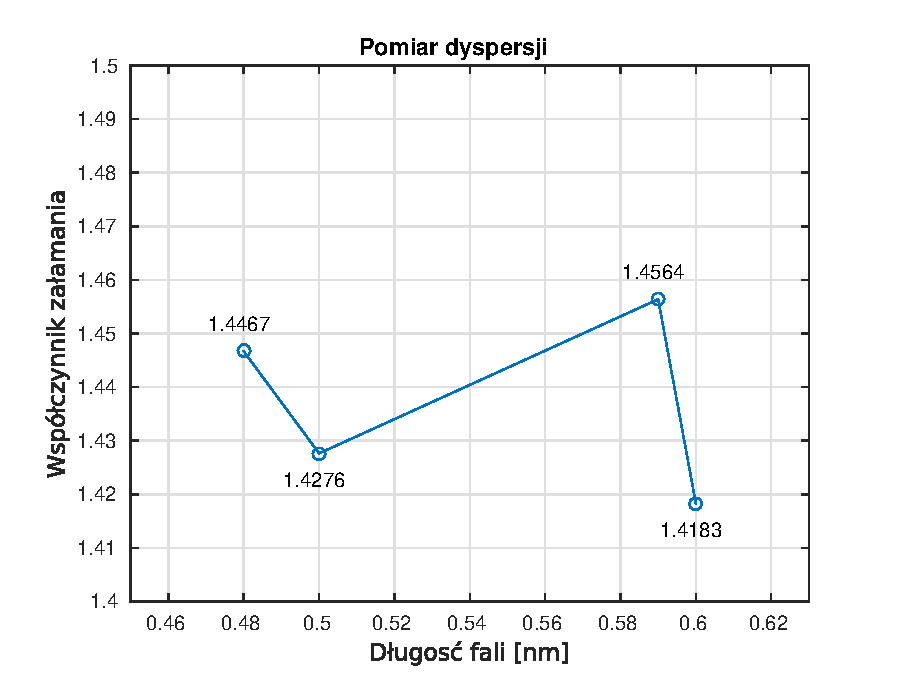
\includegraphics[width=.8\linewidth]{untitled.eps}
\end{Figure}

\end{document}